\documentclass{article}
\usepackage[T1]{fontenc}
\usepackage{lmodern}
\usepackage{graphicx}
\usepackage{amsmath,amssymb}
\usepackage[a4paper,margin=2cm]{geometry}
\usepackage[absolute,overlay]{textpos}
\setlength{\TPHorizModule}{1mm}
\setlength{\TPVertModule}{1mm}
\usepackage[indonesian]{babel}
\usepackage{hyperref}
\setlength{\emergencystretch}{2em}
% unit: Halaman 12

\begin{document}

% === Halaman 12 (llm) ===

\vspace{164.54mm}

CrypTool-Online\newline Cryptography for everybody\newline\newline N-gram tables

% deskripsi: Tabel analisis N-gram yang menunjukkan peringkat (Rank), karakter 1-gram, jumlah absolut (Abs.), dan nilai relatif (Rel.) untuk sekumpulan karakter.
% bbox normalisasi: [0.1220, 0.3160, 0.4950, 0.8700]
\begin{textblock*}{78.33mm}(25.62mm,93.85mm)
\noindent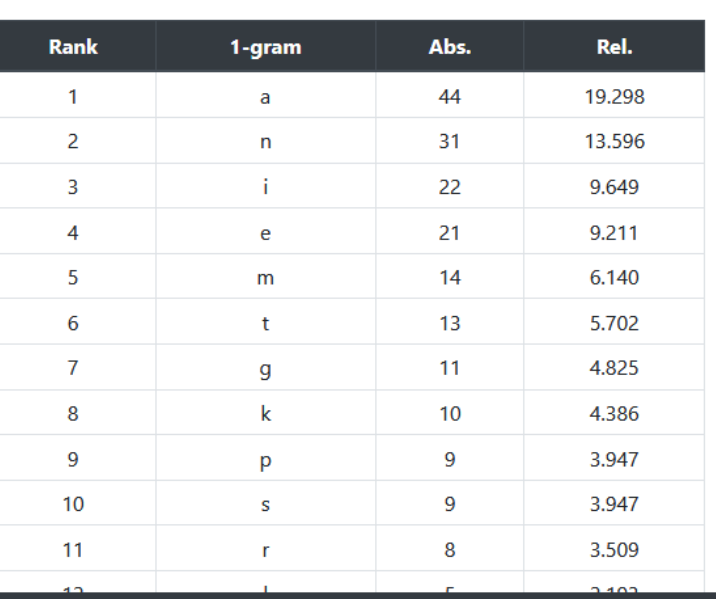
\includegraphics[width=78.33mm,height=164.54mm]{../../images/llm/page_012_img_01.png}%
\end{textblock*}

\end{document}
